\documentclass[class=article,10pt,crop=false]{standalone}
\usepackage{preamble}

\begin{document}
\begin{multicols}{2}[\section{Mechanics and special relativity}]
\subsection{Mechanics}
\subsubsection{Kinematics}
\begin{concept}[Movement equations]
$$\boldsymbol{r}(t)=x(t)\boldsymbol{e}_x+y(t)\boldsymbol{e}_y+z(t)\boldsymbol{e}_z,$$ where $x(t)$, $y(t)$, $z(t)$ are the movements equations of a particle.
\end{concept}
\begin{concept}[Average and instantaneous velocity]
Consider a particle is at point $r(t_1)$ in the instant $t_1$ and at point $r(t_2)$ in the instant $t_2$. Then the \textit{average velocity over the time interval $\Delta t=t_2-t_1$} is $$\boldsymbol{v}_\text{avg}=\frac{\Delta\boldsymbol{r}}{\Delta t},$$ where $\Delta r=r(t_2)-r(t_1)$. If we take the limit when $\Delta t\to0$, we get the \textit{instantaneous velocity}: $$\boldsymbol{v}(t)=\lim_{\Delta t\to 0}\frac{\Delta\boldsymbol{r}}{\Delta t}=\dot{\boldsymbol{r}}(t)=\dot{x}(t)\boldsymbol{e}_x+\dot{y}(t)\boldsymbol{e}_y+\dot{z}(t)\boldsymbol{e}_z$$
\end{concept}
\begin{concept}[Speed]
The \textit{speed} of a particle moving at a velocity $\boldsymbol{v}(t)$ is $$v(t)=\|\boldsymbol{v}(t)\|.$$
\end{concept}
\begin{concept}[Average and instantaneous acceleration]
Consider a particle moving at a velocity $v(t_1)$ in the instant $t_1$ and at a velocity $v(t_2)$ in the instant $t_2$. Then the \textit{average acceleration over the time interval $\Delta t=t_2-t_1$} is $$\boldsymbol{a}_\text{avg}=\frac{\Delta\boldsymbol{v}}{\Delta t},$$ where $\Delta v=v(t_2)-v(t_1)$. If we take the limit when $\Delta t\to0$, we get the \textit{instantaneous acceleration}: $$\boldsymbol{a}(t)=\lim_{\Delta t\to 0}\frac{\Delta\boldsymbol{v}}{\Delta t}=\ddot{\boldsymbol{r}}(t)=\ddot{x}(t)\boldsymbol{e}_x+\ddot{y}(t)\boldsymbol{e}_y+\ddot{z}(t)\boldsymbol{e}_z$$
\end{concept}
\begin{concept}[Uniform linear motion]
Consider a particle moving at a constant speed $v$ along a straight line. If at time $t=0$ it is at position $x_0$, then $$x(t)=x_0+vt.$$
\end{concept}
\begin{concept}[Uniform accelerated linear motion]
Consider a particle moving at a constant acceleration $a$ along a straight line. If at time $t=0$ it is at position $x_0$ with velocity $v_0$, then $$\cdot{x}(t)=v_0+at,\quad x(t)=x_0+v_0t+\frac{1}{2}at^2.$$
\end{concept}
\begin{concept}[Circular movement in polar coordinates]
Since we know $x=r\cos\varphi$ and $y=r\sin \varphi$ we can define the polar unit vectors as
\begin{gather*}
    \boldsymbol{e}_r=\cos\varphi\boldsymbol{e}_x+\sin\varphi\boldsymbol{e}_y\\
    \boldsymbol{e}_\varphi=-\sin\varphi\boldsymbol{e}_x+\cos\varphi\boldsymbol{e}_y
\end{gather*}
The equation of the circular movement are the following: $$\boldsymbol{r}(t)=r\boldsymbol{e}_r,\;\boldsymbol{v}(t)=r\dot{\varphi}(t)\boldsymbol{e}_\varphi,\;\boldsymbol{a}(t)=r\ddot{\varphi}(t)\boldsymbol{e}_\varphi-r\left[\dot{\varphi}(t)\right]^2\boldsymbol{e}_r,$$ where we have supposed that $r$ is constant. We define the \textit{angular velocity $\omega(t)$} as $\omega(t):=\dot{\varphi}(t)$ and the \textit{angular acceleration $\alpha(t)$} as $\alpha(t):=\ddot{\varphi}(t)$. The first term of $\boldsymbol{a}(t)$ is called the tangential acceleration and its magnitude is $a_t:=r\alpha$; the second one is called the normal acceleration and its magnitude is $a_n:=r\omega^2=\frac{v^2}{r}$.
\end{concept}
\begin{concept}[General motion in two dimensions]
Consider a particle moving along the trajectory $\boldsymbol{r}(t)$. We define Frenet vectors as:
\begin{enumerate}
    \item First Frenet vector: $\displaystyle\boldsymbol{e}_1(t)=\frac{\dot{\boldsymbol{r}}(t)}{\|\dot{\boldsymbol{r}}(t)\|}$
    \item Second Frenet vector: $\displaystyle\boldsymbol{e}_2(t)=\frac{\dot{\boldsymbol{e}}_1(t)}{\|\dot{\boldsymbol{e}}_1(t)\|}$
\end{enumerate}
Note that the first vector is tangent to the trajectory at each point and the second one is normal to the trajectory at each point.\newline From this definition we have that $$\dot{\boldsymbol{r}}(t)=v(t)\boldsymbol{e}_1,\quad\ddot{\boldsymbol{r}}(t)=a_t(t)\boldsymbol{e}_1+a_n(t)\boldsymbol{e}_2(t).$$ We also define the \textit{curvature $\kappa(t)$} and \textit{radius of curvature $R(t)$} as $$\frac{1}{\kappa(t)}=R(t):=\frac{\|\dot{\boldsymbol{r}}(t)\|}{\|\dot{\boldsymbol{e}}_1(t)\|}.$$ Finally, the normal acceleration is $$a_n(t)=\frac{\left[v(t)\right]^2}{R(t)}.$$
\end{concept}
\begin{concept}[General motion in two dimensions - curvature]
Consider a particle moving along a two-dimensional trajectory and let $\Delta\varphi$ be the angle the trajectory has curved when traveling a distance $\Delta s$. Then the \textit{average curvature along $\Delta s$} is $$\kappa_\text{avg}=\frac{\Delta \varphi}{\Delta s}$$. If we take the limit when $\Delta s\to 0$ we have: $$\kappa=\lim_{\Delta s\to 0}\frac{\Delta \varphi}{\Delta s}=\frac{d\varphi}{ds}.$$
\end{concept}
\begin{concept}[General motion in two dimensions - arc length]
The total distance traveled by a particle moving along a curve $c$ between the instants $t_1$ and $t_2$ is $\boldsymbol{r}(t)$ is $$L=\int_{t_1}^{t_2}v(t)dt$$
\end{concept}
\begin{concept}[Projectile motion]
Equations of a projectile motion as in figure \textcolor{green}{POSAR FIGURA}
\begin{gather*}
    x(t)=x_0+v_0\cos\varphi t\\
    y(t)=y_0+v_0\sin\varphi t-\frac{1}{2}gt^2\\
    v_x(t)=v_0\cos\varphi\\
    v_y(t)=v_0\sin\varphi-gt
\end{gather*}
\end{concept}
\subsubsection{Dynamics}
Segona llei de Newton: $$\frac{\boldsymbol{F}(\boldsymbol{r}(t),\dot{\boldsymbol{r}}(t),t)}{m}=\ddot{\boldsymbol{r}}(t)$$
Força gravitatòria: $$\boldsymbol{F}=-G\frac{Mm}{r^2}\hat{r}$$
Força elàstica: $$F_e=-kx$$
Oscil·lador:
\begin{gather*}
    F_e=ma\iff\ddot{x}(t)+\omega^2x(t)=0\\
    x(t)=A\cos(\omega t+\phi)\\
    \dot{x}(t)=-\omega A\sin(\omega t+\phi)\\
    \ddot{x}(t)=-\omega^2 A\cos(\omega t+\phi)=-\omega^2x(t)\\
    \omega=\sqrt{\frac{k}{m}}\qquad T=\frac{2\pi}{\omega}\qquad\nu=\frac{1}{T}
\end{gather*}
Coeficients de fregament:
\begin{itemize}
    \item $\mu_e=$ coeficient estàtic de fregament.
    \item $\mu_c=$ coeficient cinètic de fregament.
\end{itemize} 
Força de fregament: $$F_f=\left\{
    \begin{array}{rcl}
    F & \text{si} & F\leq\mu_eF_{\!_N} \\
    \mu_cF_{\!_N} & \text{si} & F>\mu_eF_{\!_N}
    \end{array}\right.$$
    {on $F$ és la força aplicada a l'objecte i $F_{\!_N}$ la força normal.}\newline
Forces inercials: força fictícia per a sistemes de referència no inercials. $$\boldsymbol{F}(t)+\boldsymbol{F}_{\text{iner}}(t)=m\ddot{\boldsymbol{r}}\,'(t)$$ {on $\boldsymbol{F}_{\text{iner}}(t)\equiv-m\ddot{\boldsymbol{R}}(t)$ i $\boldsymbol{R}(t)$ és l'equació del moviment d'un sistema de referència respecte de l'altre.}\newline
Transformacions de Galileo:
\begin{align*}
    x'&=x-Vt & v_x'&=v_x-V\\
    y'&=y & v_y'&=v_y\\
    z'&=z & v_z'&=v_z\\
    t'&=t
\end{align*} {on $V$ és la velocitat de $S'$ respecte $S$.}
\subsubsection{Statics}
\begin{concept}[Linear momentum of a particle] Consider a particle of mass $m$ moving a t a velocity of $v$. We define its \textit{linear momentum} as:
$$\boldsymbol{p}=m\boldsymbol{v}$$
\end{concept}
\begin{concept}[Newton's second law]
$$\boldsymbol{f}=\frac{d\boldsymbol{p}}{dt}.$$
\end{concept}
\begin{concept}[Linear momentum of a system of particles]
Consider a system of $N$ particles which interact with themselves (internal forces) and also with external forces. The total force $\boldsymbol{f}_a$ applied to the particle $a$ is $$\boldsymbol{f}_a=\boldsymbol{f}_a^\text{ext}+\sum_{\substack{b=1\\b\ne a}}^N\boldsymbol{f}_{b\to a},$$ where $\boldsymbol{f}_{b\to a}$ is the internal force that particle $b$ makes on particle $a$ and $\boldsymbol{f}_a^\text{ext}$ is the external force applied to $a$. Then the \textit{linear momentum of the system} is $$\boldsymbol{P}=\sum_{a=1}^N\boldsymbol{p}_a.$$ If $\boldsymbol{F}^\text{ext}=\sum_{a=1}^N\boldsymbol{f}_a^\text{ext}$ is the total external force applied to the system, we have: $$\dot{P}=\boldsymbol{F}^\text{ext}$$
\end{concept}
\begin{concept}[Center of masses]
The \textit{center of masses} of a system of $N$ particles is: $$\boldsymbol{R}=\frac{1}{M}\sum_{a=1}^Nm_a\boldsymbol{r}_a,$$ where $\displaystyle M=\sum_{a=1}^Nm_a$. Differentiating the last equality we get $$M\dot{\boldsymbol{R}}=\boldsymbol{P},\quad
M\ddot{\boldsymbol{R}}=\dot{\boldsymbol{P}}=\boldsymbol{F}^\text{ext}.$$
If the mass distribution is continuous with the density $\rho(\boldsymbol{r})$ within a solid $\Omega$, the center of mass is $$\boldsymbol{R}=\frac{1}{M}\iiint_\Omega\rho(\boldsymbol{r})\boldsymbol{r}dV,$$ where $\displaystyle M=\iiint_\Omega\rho(\boldsymbol{r})dV$.
\end{concept}
\begin{concept}[Angular momentum]
Consider a particle with linear momentum $\boldsymbol{p}$ situated at position $\boldsymbol{r}$ with respect to the origin $O$. We define its \textit{angular momentum} as $$\boldsymbol{l}=\boldsymbol{r}\times\boldsymbol{p}.$$ The angular momentum of a system of $N$ particles is $$\boldsymbol{L}=\sum_{a=1}^N\boldsymbol{l}_a.$$
\end{concept}
\begin{concept}[Torque]
Consider a particle at position $\boldsymbol{r}$ with respect to the origin $O$ and let $\boldsymbol{f}$ be a force acting to on the particle. We define its \textit{torque} as $$\boldsymbol{m}=\boldsymbol{r}\times\boldsymbol{f}.$$ The torque of a system of $N$ particles is $$\boldsymbol{M}=\sum_{a=1}^N\boldsymbol{m}_a.$$
\end{concept}
\begin{concept}[Conservation of angular momentum]
$$\dot{\boldsymbol{l}}=\boldsymbol{m},\quad\dot{\boldsymbol{L}}=\boldsymbol{M}^\text{ext},$$where $\boldsymbol{M}^\text{ext}$ is the net torque caused by external forces So if $\boldsymbol{M}^\text{ext}=0$, then $\dot{\boldsymbol{L}}$ and therefore $\boldsymbol{L}$ is constant.
\end{concept}
\begin{concept}[Mechanical equilibrium]
The necessary conditions of mechanical equilibrium are $$\boldsymbol{F}^\text{ext}=0,\quad\boldsymbol{M}^\text{ext}=0$$
\end{concept}
\subsubsection{Work and energy}
\begin{concept}[Work]
The \textit{work} of a constant force $\boldsymbol{f}$ acting on a particle that moves in a straight line is $$ W=\boldsymbol{f}\cdot\Delta\boldsymbol{r}.$$ If the force is not necessary constant and the particle moves along a curve $c$, we have $$W=\int_c\boldsymbol{f}\cdot d\boldsymbol{r}.$$
\end{concept}
\begin{concept}[Power]
In general, the \textit{power} is defined as $$P=\frac{dW}{dt}.$$ In general, if $\Delta W$ is the amount of work performed during a period of time of duration $\Delta t$, the \textit{average power} is $$P=\frac{\Delta W}{\Delta t}.$$ If we take the limit when $\Delta t\to 0$, we obtain the \textit{instantaneous power}: $$P=\boldsymbol{f}\cdot\boldsymbol{v}.$$ This formula is valid for any general situation.
\end{concept}
\begin{concept}[Kinetic energy]
The \textit{kinetic energy} of a particle of mass $m$ moving at a velocity $\boldsymbol{v}$ is $$K=\frac{1}{2}m\|\boldsymbol{v}\|^2=\frac{1}{2}mv^2$$
\end{concept}
\begin{theorem}[Work-kinetic energy theorem]
$$W=\Delta K$$
\end{theorem}
\begin{definition}[Conservative forces]
A force is \textit{conservative} if for any path $c$ connecting points $A$ and $B$, the work necessary to move a particle from $A$ to $B$ does not depend on $c$.
\end{definition}
\begin{concept}[Potential energy]
If a force $\boldsymbol{f}$ is conservative, we define the potential energy as $$U(\boldsymbol{r})=-\int_{\boldsymbol{r}_0}^{\boldsymbol{r}}\boldsymbol{f}\cdot d\boldsymbol{r},$$ where $\boldsymbol{r}_0$ is a reference point and can be chosen arbitrarily. It can be easily seen that $$W=-\Delta U.$$
\end{concept}
\begin{concept}[Mechanical energy]
The mechanical energy of a particle (with kinetic energy $K$) subjected to a conservative force of potential energy $U$ is $$E=K+U.$$
\end{concept}
\begin{concept}[Conservation of mechanical energy]
For a particle subjected to a conservative force we have $$\Delta E=0.$$ That is, $E$ is constant. If there are non-conservative forces acting on the particle we have $$\Delta E=W_{\text{nc}},$$ where $W_\text{nc}$ is the work done by non-conservative forces.
\end{concept}
\begin{concept}[Examples of potential energies]
\hfill
\begin{enumerate}
    \item Elastic potential energy of a spring: $$U=\frac{1}{2}kx^2,$$ where $x$ is the distance the spring has been stretched.
    \item Gravitational potential energy of a solid of mass $m$: $$U=-\frac{GM_Tm}{r},$$ where $M_T$ is the Earth mass, $r$ is the distance form the center of the earth to the position of the solid and $G=6,67\times 10^{-11}\;\frac{N\cdot m^2}{kg^2}$ is the gravitational constant. Note that if $r=R_T+h$, $h>0$ and $\frac{r}{R_T}=1+\frac{h}{R_T}\approx 1$, then $$U=mgh,$$ where $R_T$ is the radius of earth and $g=9,8\;m/s^2$.
\end{enumerate}
\end{concept}
\subsubsection{Rotation}
Moment d'inèrcia: $$I_e=\sum_im_i\eta_i^2$$ {on $\eta_i$ és la distància entre la posició de la partícula de massa $m_i$ i l'eix $e$.}\newline
Moment angular: $$L_e=I_e\omega$$
Sòlid rígid: $$M_e^\text{ext}=\dot{L}_e=I_e\dot{\omega}=I_e\alpha$$
Moment angular respecte del CM:$$\boldsymbol{L}_O=\boldsymbol{L}_{CM}+\boldsymbol{R}\times\boldsymbol{P}$$ {on $\boldsymbol{R}$ és la distància del $CM$ al punt $O$.}\newline
Moment d'una força respecte del CM: $$\boldsymbol{M}_O^\text{ext}=\boldsymbol{M}_{CM}^\text{ext}+\boldsymbol{R}\times\boldsymbol{F}_\text{total}^\text{ext}$$ {on $\boldsymbol{R}$ és la distància del $CM$ al punt $O$.}
$$\dot{\boldsymbol{L}}_{CM}=\boldsymbol{M}_{CM}^\text{ext}$$
Energia cinètica de rotació: $$K=\frac{1}{2}MV^2+\frac{1}{2}I_{CM}\omega^2$$
Teorema d'Steiner: $$I_{e'}=I_e+Ma^2$$ {on $a$ és la distància entre els eixos $e$ i $e'$.}
\subsection{Special relativity}
\begin{definition}
A \textit{inertial frame of reference} is a frame of reference in which a particle remains at rest or in uniform linear motion.
\end{definition}
\begin{concept}[First postulate (Principle of relativity)]
The laws of physics take the same form in all inertial frames of reference.
\end{concept}
\begin{concept}[Second postulate]
The speed of light $c$ is a constant, independent of the relative motion of the source.
\end{concept}
\begin{concept}[Galilean transformations]
Consider coordinates $(x,y,z,t)$ and $(x',y',z',t')$ of a single arbitrary event measured in two coordinate systems $S$ and $S'$, in uniform relative motion ($S'$ is moving at velocity $v$ respect to $S$) in their common $x$ and $x'$ directions and  with their spatial origins coinciding at time $t=t'=0$. Then:
\begin{align*}
    x'&=x-vt & u_x'&=u_x-v\\
    y'&=y & u_y'&=u_y\\
    z'&=z & u_z'&=u_z\\
    t'&=t & &
\end{align*}
where $\boldsymbol{u}=(u_x,u_y,u_z)$ and $\boldsymbol{u'}=(u_x',u_y',u_z')$ are the velocities of the systems $S$ and $S'$.
\end{concept}
\textcolor{green}{POSAR FOTO}% https://tex.stackexchange.com/questions/239980/tikz-get-position-node-of-an-arrow-head
\begin{concept}[Lorentz factor]
$$\gamma=\frac{1}{\sqrt{1-\beta^2}},$$ where $\beta=v/c$
\end{concept}
\begin{concept}[Time dilation]
Consider two frames of reference in uniform relative motion with velocity $v$ such that one of them has a clock. If $\Delta t_0$ is the time interval between two events made in the same location and measured in the frame in which the clock is at rest (\textit{proper time}), then the time measured by the other frame is
$$\Delta t=\gamma\Delta t_0.$$
\end{concept}
\begin{concept}[Length contraction]
Consider two frames of reference in uniform relative motion with velocity $v$ such that one of them has an object. If $L_0$ is length of the object measured instantaneously in the frame in which the object is at rest (\textit{proper length}), then the length measured by the other frame is
$$L=\frac{L_0}{\gamma}.$$
\end{concept}
\begin{concept}[Lorentz transformations]
Consider coordinates $(x,y,z,t)$ and $(x',y',z',t')$ of a single arbitrary event measured in two coordinate systems $S$ and $S'$, in uniform relative motion ($S'$ is moving at velocity $v$ with respect to $S$) in their common $x$ and $x'$ directions and  with their spatial origins coinciding at time $t=t'=0$. Then:
\begin{align*}
    x'&=\gamma(x-\beta ct) & x&=\gamma(x'+\beta ct')\\
    y'&=y & y&=y'\\
    z'&=z & z&=z'\\
    ct'&=\gamma(ct-\beta x) & ct&=\gamma(ct'+\beta x')
\end{align*}
\end{concept}
\begin{concept}[Lorentz transformations of velocities]
In a situation similar to the previous one, if an object is moving at a velocity $\boldsymbol{u}=(u_x,u_y,u_z)$ in $S$ and $\boldsymbol{u'}=(u_x',u_y',u_z')$ in $S'$, we have:
\begin{align*}
    u_x'&=\frac{u_x-v}{1-u_xv/c^2} & u_x&=\frac{u_x'+v}{1+u_x'v/c^2}\\
    u_y'&=\frac{u_y}{\gamma \left(1-u_xv/c^2\right)} & u_y&=\frac{u_y'}{\gamma \left(1+u_xv/c^2\right)}\\
    u_z'&=\frac{u_z}{\gamma \left(1-u_xv/c^2\right)} & u_z&=\frac{u_z'}{\gamma \left(1+u_xv/c^2\right)}
\end{align*}
\end{concept}
\begin{concept}[Matrix form of Lorentz transformations]
We can write the Lorentz transformations as: 
$$\begin{pmatrix}
x'\\
ct'
\end{pmatrix}=\begin{pmatrix}
\gamma & -\beta\gamma\\
-\beta\gamma & \gamma
\end{pmatrix}\begin{pmatrix}
x\\
ct
\end{pmatrix}.$$ If $$\Lambda:=\begin{pmatrix}
\gamma & -\beta\gamma\\
-\beta\gamma & \gamma
\end{pmatrix},\text{ then }\Lambda^{-1}=\begin{pmatrix}
\gamma & \beta\gamma\\
\beta\gamma & \gamma
\end{pmatrix}$$ and we obtain the inverse transformations.
\end{concept}
\begin{concept}[Lorentz invariant]
The factor $s^2$, defined as follows, is invariant in any inertial frame of reference. $$s^2=c^2t^2-x^2-y^2-z^2.$$
\end{concept}
\begin{concept}[Types of events]
There are three types of events: \textit{timelike}, \textit{lightlike} and \textit{spacelike}.
\begin{itemize}
    \item $s^2>0\implies timelike$,
    \item $s^2=0\implies lightlike$,
    \item $s^2<0\implies spacelike$.
\end{itemize}
Timelike and lightlike events are in causal relation with the origin (it is possible to send a light signal from the origin to the point or vice versa), while \textit{spacelike} event not.
\end{concept}
\begin{figure}[ht]
    \centering
    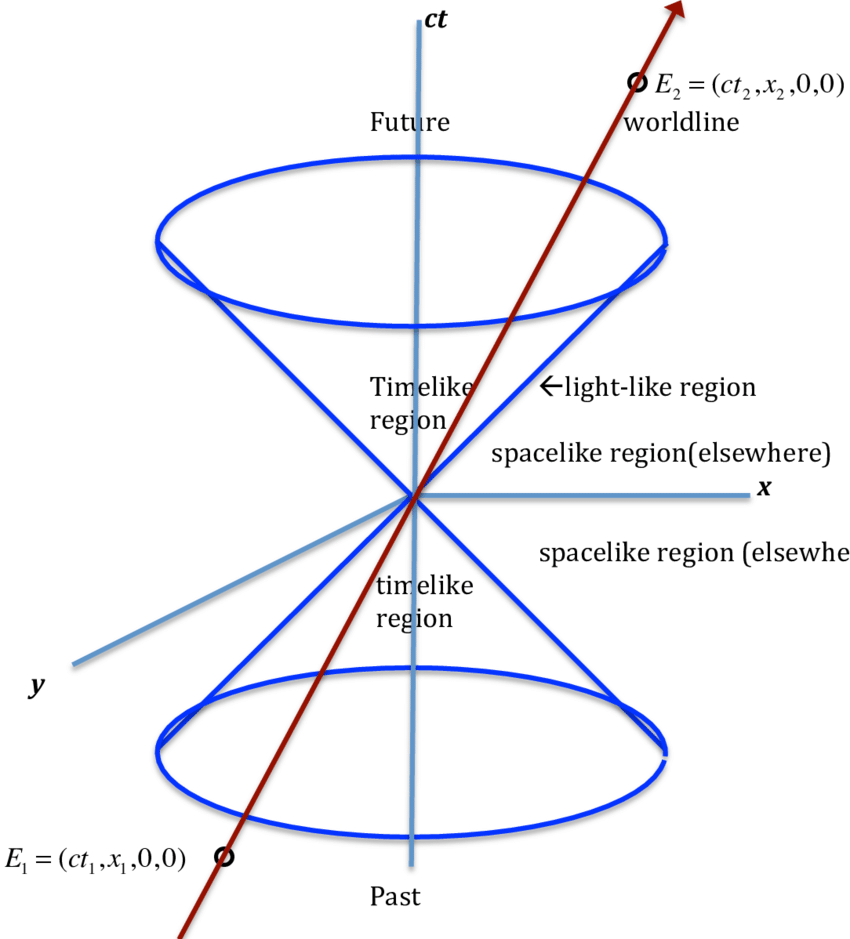
\includegraphics[width=4cm]{Physics/1st/Mechanics_and_special_relativity/Images/mink.png}
    \caption{Con del passat i del futur.}
\end{figure}
\textcolor{green}{POSAR DIAGRAMES DE MINKOWSKI}
\begin{concept}[Relativistic Doppler effect]
Suppose a frame of reference where the receiver is at rest and the source is moving at speed $\beta$ forming an angle $\phi$ with the light direction (measured in receiver frame). Then, 
\begin{gather}
    \label{dopp1}\nu_R=\frac{\nu_E}{\gamma(1-\beta\cos\phi)}\\
    \lambda_R=\gamma\lambda_E(1-\beta\cos\phi)
\end{gather} where $\nu_E$ is the frequency measured by the source and $\nu_E$ is the frequency measured by the receiver, and analogously with $\lambda_E$ and $\lambda_R$.\newline Relation between the angles $\phi$ and $\phi'$, where $\phi'$ is the angle between the velocity and the light direction measured in source frame: 
$$\tan\frac{\phi'}{2}=\sqrt{\frac{1+\beta}{1-\beta}}\tan\frac{\phi}{2}.$$
\end{concept}
\begin{figure}[ht]
    \centering
    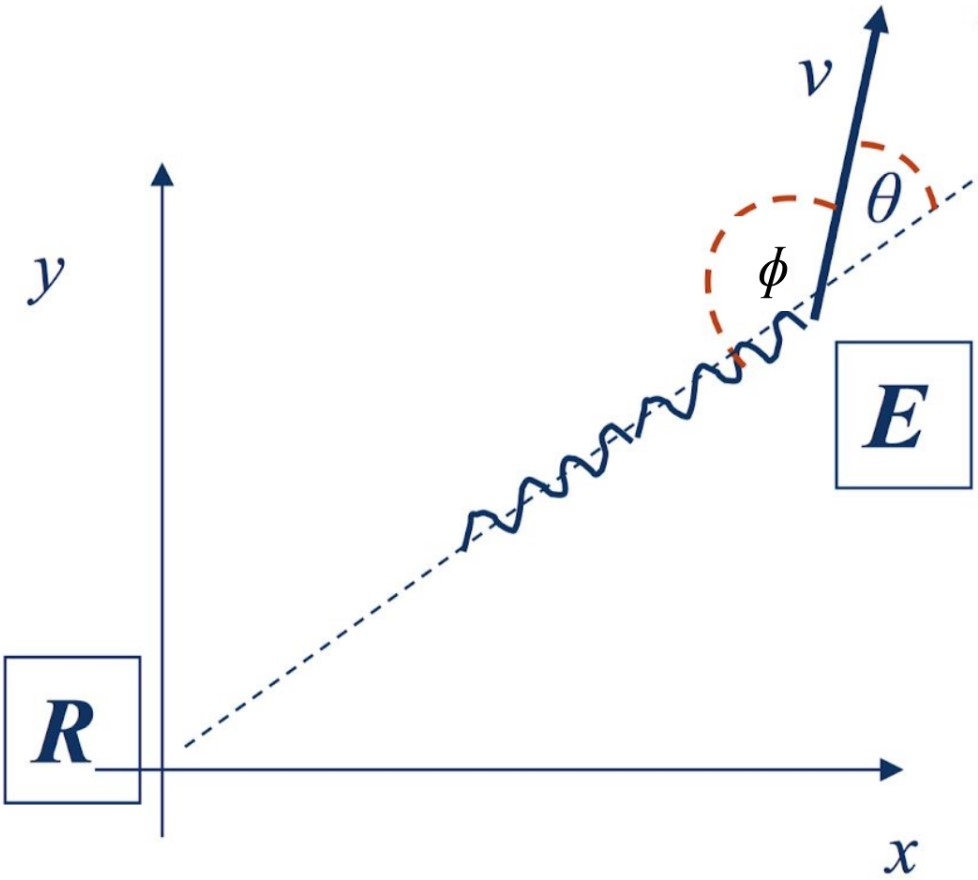
\includegraphics[width=4cm]{Physics/1st/Mechanics_and_special_relativity/Images/dop.jpg}
    \caption{Cas general d'efecte Doppler relativista.}
\end{figure}
\begin{concept}[Relativistic longitudinal Doppler effect]
We have two cases to consider:
\begin{itemize}
    \item If the source moves away, that is making $\phi=\pi$ in equation \eqref{dopp1} (\textit{Redshift}):
   $$\nu_R=\nu_E\sqrt{\frac{1-\beta}{1+\beta}}.$$
    \item If the source moves closer, that is making $\phi=0$ in equation \eqref{dopp1} (\textit{Blueshift}):
   $$\nu_R=\nu_E\sqrt{\frac{1+\beta}{1-\beta}}.$$
\end{itemize}
\end{concept}
\begin{concept}[Relativistic transverse Doppler effect]
Making $\phi=\pi/2$ in equation \eqref{dopp1}:$$\nu_R=\nu_E/\gamma.$$
\end{concept}
\begin{concept}[Relativistic mass]
If $m_0$ is the mass of an object at rest, then the mass of an object at a velocity $\beta$ is $$m=\gamma m_0.$$ The mass $m_0$ is invariant.
\end{concept}
\begin{concept}[Relativistic momentum]
The relativistic momentum is given by $$\boldsymbol{p}=\gamma m_0\boldsymbol{u}.$$
\end{concept}
\begin{concept}[Relativistic energy]
The relativistic energy of a particle is: $$E=mc^2=\gamma m_0c^2.$$ On the other hand, $E=K+m_0c^2$, where $K$ is the kinetic energy of a particle and $m_0c^2$ its rest energy. Also we can express the energy of a particle in terms of its momentum:
$$E=mc^2=\sqrt{p^2c^2+m_0^2c^4}.$$
\end{concept}
\begin{concept}[Photon energy and momentum]
$$E=h\nu,\quad\boldsymbol{p}=\frac{h\nu}{c}\boldsymbol{n},\quad E=cp,$$ where $\boldsymbol{n}$ is the movement direction of the photon.
\end{concept}
\begin{concept}[Energy-momentum Lorentz transformations]
\begin{align*}
    E'&=\gamma(E-\beta cp_x) & E&=\gamma(E'+\beta cp_x')\\
    cp_x'&=\gamma(cp_x-\beta E) & cp_x&=\gamma(cp_x'+\beta E')\\
    p_y'&=p_y & p_y&=p_y'\\
    p_z'&=p_z & p_z&=p_z'
\end{align*}
\end{concept}
\begin{concept}[Compton scattering]
Consider a photon with wavelength $\lambda$ colliding with a particle at rest. As a result of the collision, the photon energy decrease and therefore its wavelength increase (let's say the scattered photon has wavelength $\lambda'$). If the scattered photon is moving at an angle $\theta$ with respect to initial direction, we have
\end{concept}
$$\lambda'-\lambda=\frac{h}{m_0c}(1-\cos\theta).$$
where $m$ is the mass at rest of the particle (usually an electron).
\begin{figure}[ht]
    \centering
    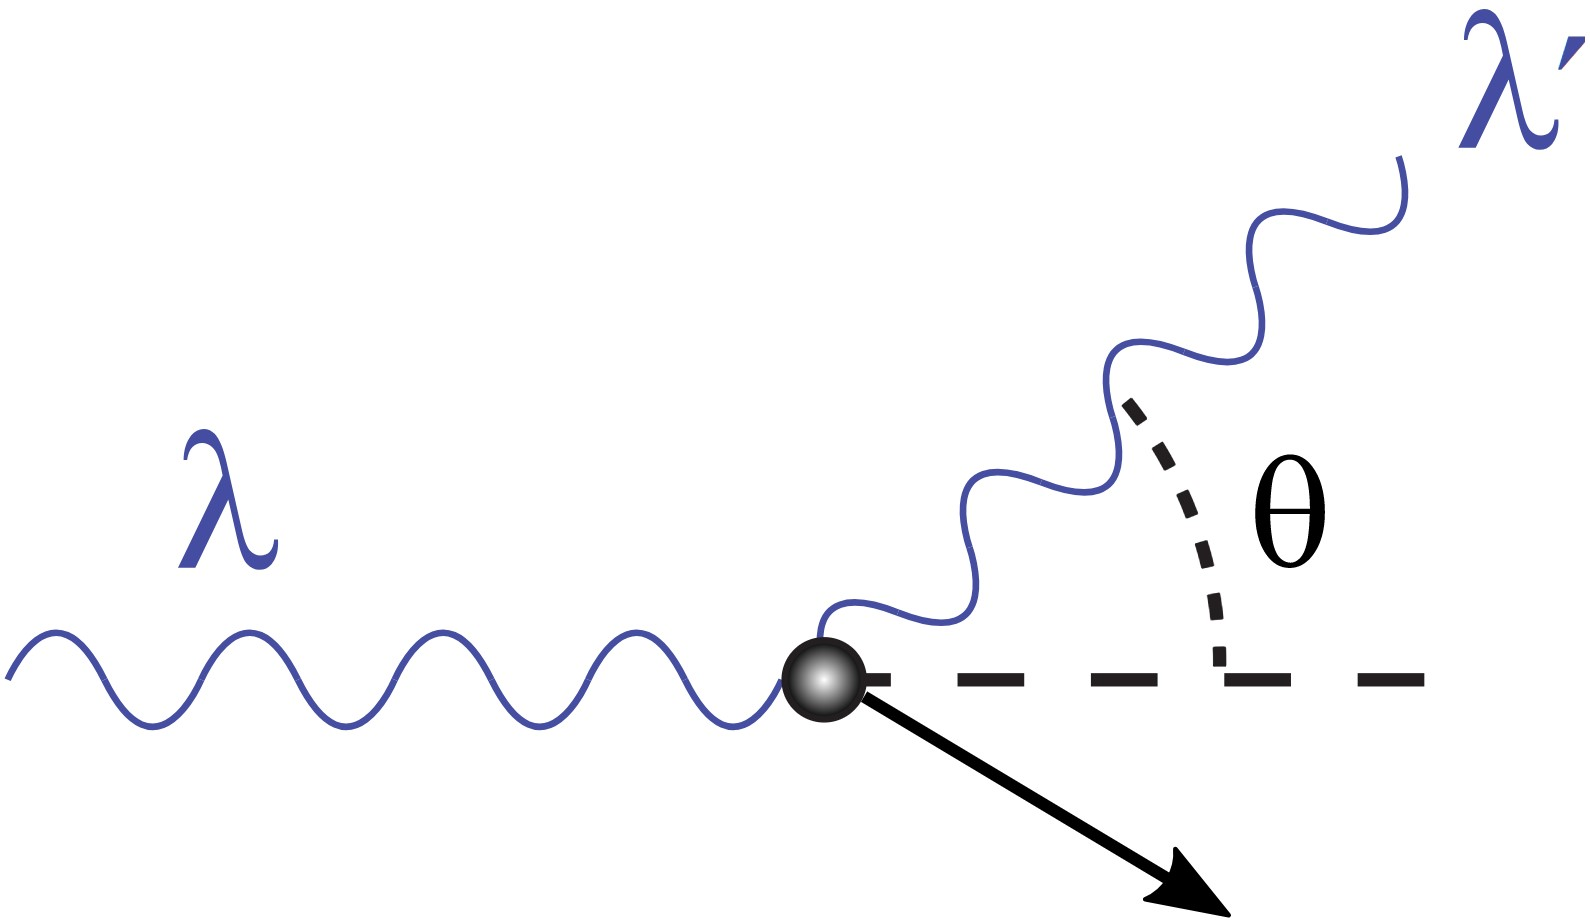
\includegraphics[width=4cm]{Physics/1st/Mechanics_and_special_relativity/Images/comp.jpg}
    \caption{Efecte Compton. Normalment la par\-tí\-cu\-la de massa sol ser un electró.}
\end{figure}
\subsection{Fluids}
\begin{definition}
A \textit{fluid} is a substance that continually flows under an applied external force.
\end{definition}
\begin{definition}
The \textit{viscosity} of a fluid is a measure of its resistance to deformation at a given rate. We say a fluid is \textit{ideal} if we don't consider viscosity.
\end{definition}
\begin{concept}[Density]
The density of a fluid is $$\rho=\frac{m}{V}.$$ The density depends on temperature and pressure.\footnote{This variation is typically small for solids and liquids but much greater for gases.}
\end{concept}
\begin{definition}
A fluid is said to be \textit{incompressible} if its density doesn't varies with the pressure. 
\end{definition}
\begin{concept}[Pressure]
Consider a point $x$ and a small sphere centered at $x$. Then the pressure $p(x)$ at point $x$ is $$p(x)=\frac{\sum F_N}{S},$$ where $\sum F_N$ is the sum of normal forces and $S$ is the surface which the forces are applied to. The SI unit of pressure is the Pascal: $1\;Pa=1\;N/m^2$.
\end{concept}
\begin{concept}[Hydrostatic pressure]
Consider a static fluid with constant density $\rho$ and let $p_0$ be the pressure at it surface. Then, the pressure $p$ at a depth $h$ is $$p=p_0+\rho gh.$$
\end{concept}
\begin{concept}[Pascal's principle]
Any pressure applied to the surface of a fluid is transmitted uniformly throughout the fluid in all directions, in such a way that initial variations in pressure are not changed.
\end{concept}
\begin{concept}[Archimedes' principle]
Any object (of mass $m$), totally or partially immersed in a fluid or liquid, is buoyed up by a force equal to the weight of the fluid displaced by the object, that is, $$F_E:=\rho gV=mg,$$ where $F_E$ is called the \textit{buoyancy} and $V$ is the volume of the liquid displaced.\footnote{Note that if the difference $F_E-mg>0$, the object rises to the surface of the liquid; if $F_E-mg<0$, the object sinks, and if $F_E-mg=0$, the object is neutrally buoyant, that is, it remains in place without either rising or sinking.}
\end{concept}
\begin{definition}
We define the \textit{discharge of a fluid} as $$Q=Sv,$$ where $S$ is the cross-sectional area of the portion of the channel occupied by the flow and $v$ is the average flow velocity. If the velocity is not constant, then $$Q=\iint_S\boldsymbol{v}\cdot d\boldsymbol{S}.$$
\end{definition}
\begin{concept}[Continuity equation]
If we have an incompressible fluid moving through a channel, then the volume per unit of time is conserved, that is, the discharge is conserved. Mathematically, $$Q_1=Q_2.$$
\end{concept}
\begin{definition}
\textit{Laminar flow} is a fluid motion that occurs when a fluid flows in parallel layers, with no disruption between those layers. \textit{Turbulent flow} is fluid motion characterized by chaotic changes in pressure and flow velocity. 
\end{definition}
\textcolor{green}{POSAR FOTO}
\begin{concept}[Bernolli's principle]
Consider an incompressible and ideal fluid with steady laminar flow. Then, $$p+\rho gh+\frac{1}{2}\rho v^2=\text{constant},$$ where $p$ is the pressure at a point on a streamline; $h$, the elevation of the point above a reference plane, and $v$, the fluid flow speed at the chosen point.
\end{concept}
\begin{concept}[Lift force]
If the air has density $\rho$ and an object of cross-sectional area $S$ is moving at a velocity of $v$ relative to the air, then the lift force is $$F_L=\frac{1}{2}C_L\rho Sv^2,$$ where $C_L$ is the lift coefficient. From that we deduce that the minimum velocity for lifting is $$F_L=mg\implies v_\text{min}=\sqrt{\frac{2mg}{C_L\rho S}}.$$
\end{concept}
\begin{concept}[Viscosity]
Consider a fluid trapped between two plates of area $S$, one fixed and one in parallel motion at constant speed $v$. If we suppose a laminar flow, each layer of fluid moves faster than the one just below it and so this creates a friction force  resisting their relative motion. An external force $F$ is therefore required in order to keep the top plate moving at constant speed. This force is given by $$F=\eta\frac{vS}{z},$$ where $z$ is the separation between the plates and $\eta$ is the viscosity of the fluid ($[\eta]=$ Pa $\cdot$ s). 
\end{concept}
\begin{figure}[ht]
    \centering
    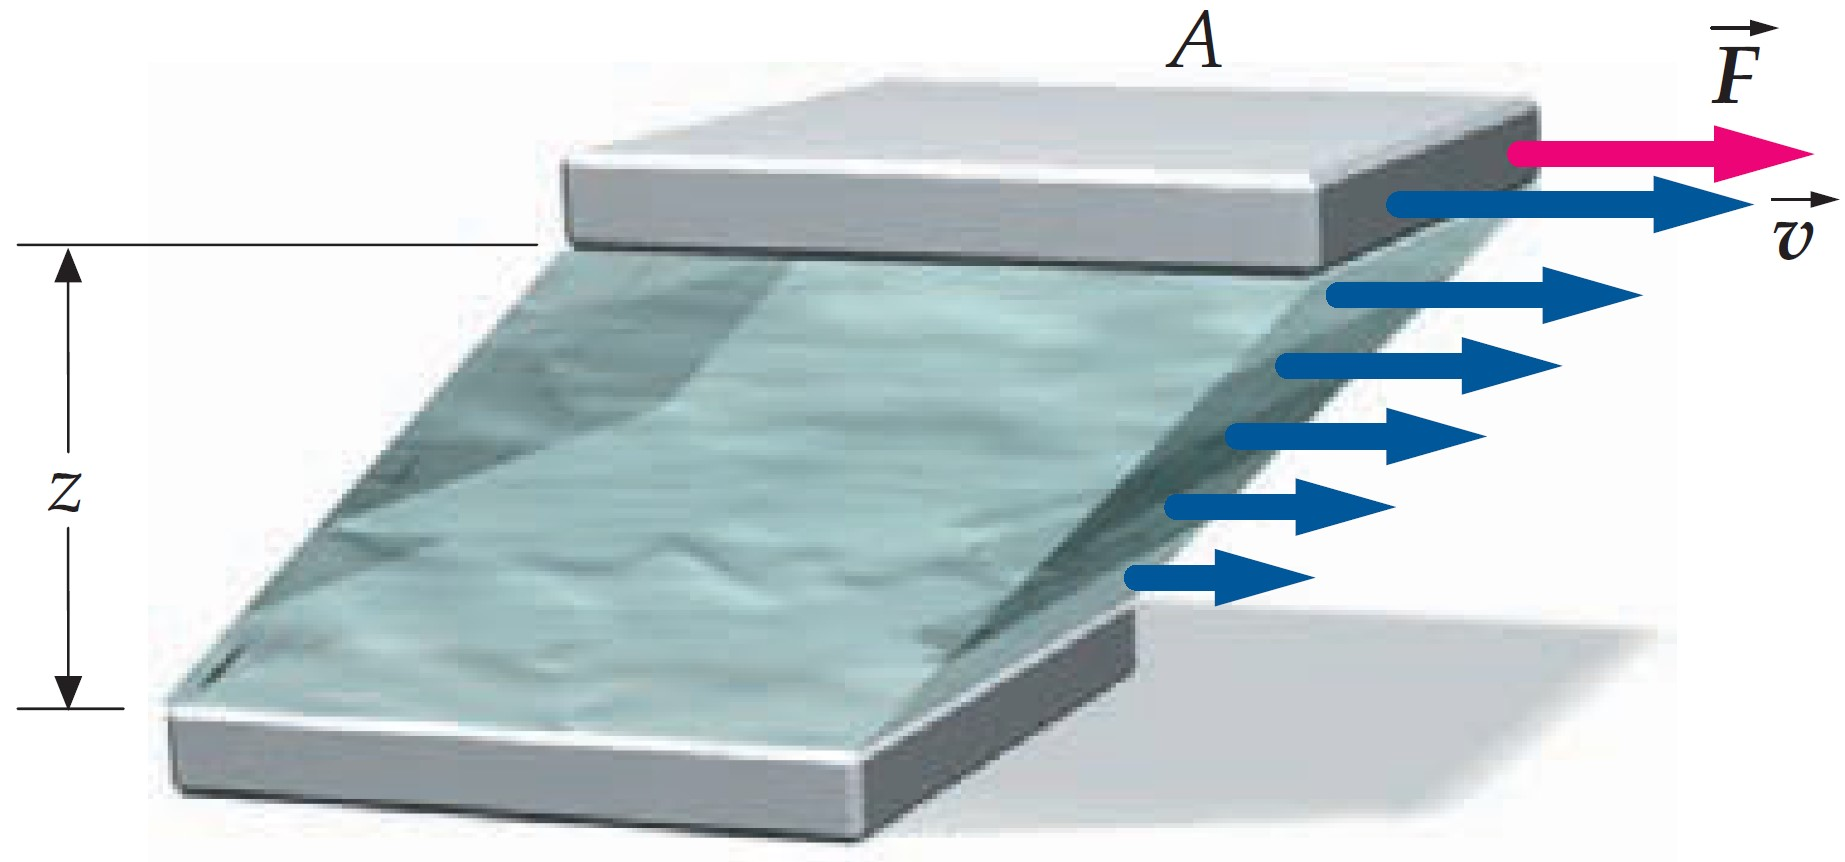
\includegraphics[width=4cm]{Physics/1st/Mechanics_and_special_relativity/Images/vis.jpg}
    \caption{Força de viscositat.}
\end{figure}
\begin{concept}[Velocity of a fluid in a channel]
Consider a fluid with viscosity $\eta$ and in laminar flow so that the the layer in contact with the wall of the channel are in rest. Following the notation on figure \textcolor{green}{POSAR FOTO} we have,
$$v(x)=\frac{p_1-p_2}{4\eta L}(r^2-x^2).$$ The average speed of the fluid is 
\begin{equation}
    v_\text{avg}=\frac{p_1-p_2}{8\eta L}r^2.
    \label{eq1}
\end{equation} Observe that $v_\text{avg}=v_\text{max}/2$.
\end{concept}
\begin{figure}[ht]
    \centering
    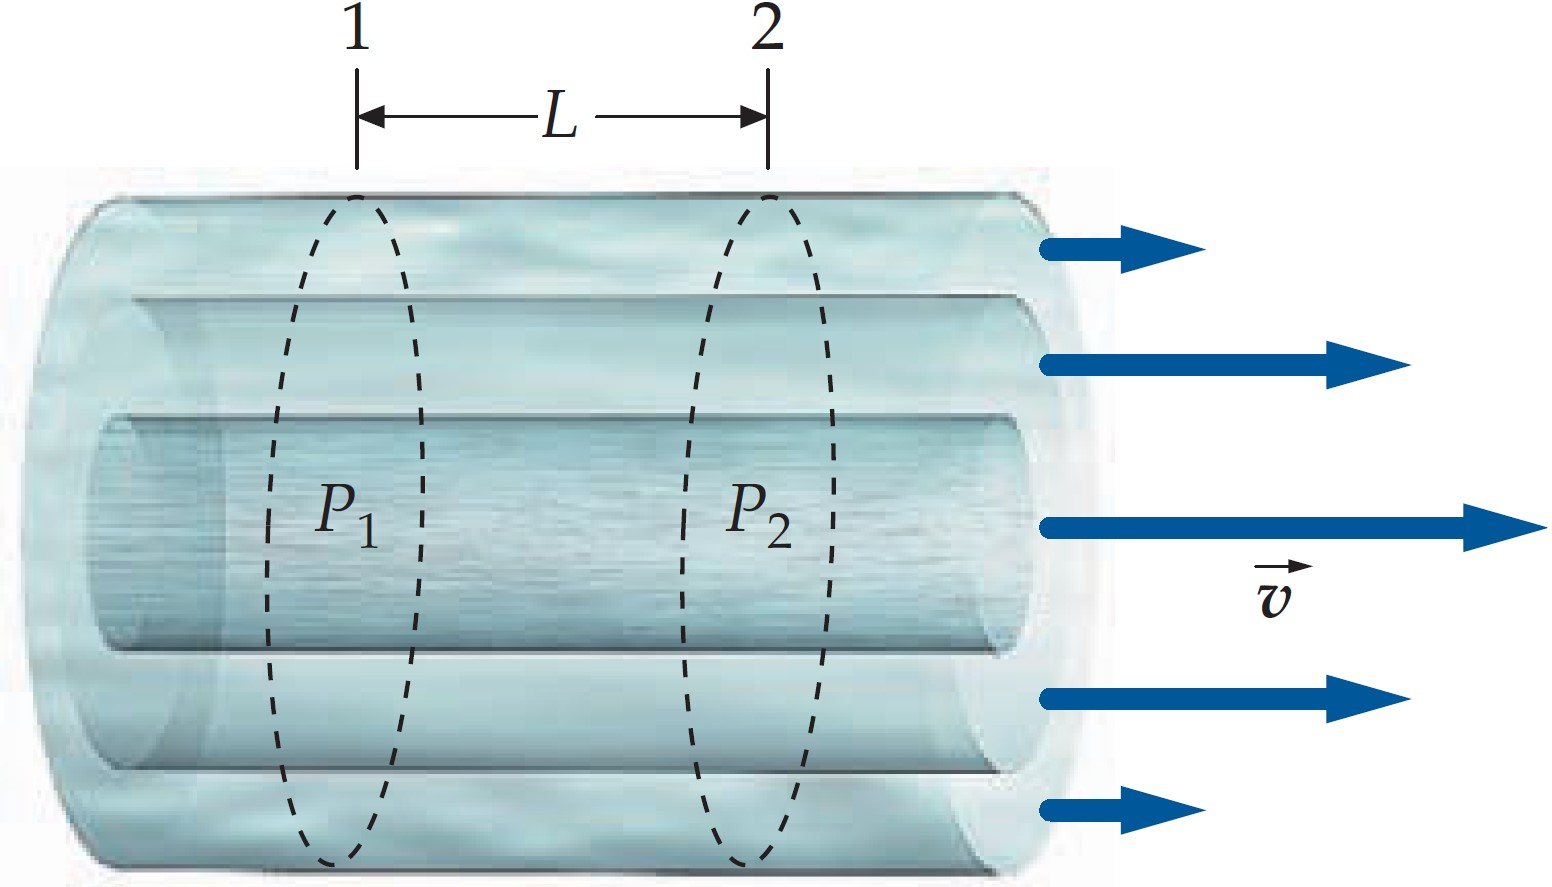
\includegraphics[width=4cm]{Physics/1st/Mechanics_and_special_relativity/Images/vis2.jpg}
    \caption{Velocitat en un fluid amb viscositat $\eta$.}
\end{figure}
\begin{concept}[Poiseuille's law]
In conditions of the equation \eqref{eq1}, we have: $$Q=Sv_\text{avg}=\frac{\pi}{8\eta }\frac{p_1-p_2}{L}r^4\implies\Delta p=\frac{8\eta}{\pi}\frac{L}{r^4}Q.$$ If we denote $\displaystyle R_f:=\frac{8\eta}{\pi}\frac{L}{r^4}$ the hydrodynamic resistance, we can write Poiseuille's law as follows: $$\Delta p=R_f Q,$$ which is an analogy of Ohm's law\footnote{In that case, $R_f$ would be the electric resistance, $Q$ the intensity of the current and $\Delta p$ the electric potential difference.}.
\end{concept}
\begin{concept}[Resistance in fluids]
\hfill\begin{itemize}
    \item In series: $$R_T=\sum_{i=1}^nR_i$$
    \item In parallel: $$\frac{1}{R_T}=\sum_{i=1}^n\frac{1}{R_i}$$
\end{itemize}
\end{concept}
\begin{concept}[Dissipated power]
$$P=\Delta pQ=R_fQ^2$$
\end{concept}
\begin{concept}[Drag forces]
An object moving at a velocity $v$ in a fluid of density $\rho$ and viscosity $\eta$ creates drag forces:
\begin{itemize}
    \item For low speeds and high viscosity, viscous forces predominate:\par 
    $$F=k\eta vr$$
    where $k=6\pi$ if the object is an sphere and $r$ is its radius.
    \item For high speeds and low viscosity, inertial forces predominate:
    $$F=\frac{1}{2}C_a\rho Sv^2,$$
    where $C_a$ is the aerodynamic coefficient and $S$ the cross-sectional area.
\end{itemize}
\end{concept}
\begin{concept}[Terminal velocity]
An object falling (by gravity) inside a fluid attains a maximum velocity (terminal velocity) when its weight equals the drag force. We have two cases to consider:
\begin{itemize}
    \item For viscous forces: $$v_t=\frac{mg}{k\eta r}$$
    \item For inertial forces: $$v_t=\sqrt{\frac{2mg}{C_a\rho S}}$$
\end{itemize}
\end{concept}
\begin{concept}[Reynolds number]
The Reynolds number helps to predict flow patterns in different fluid flow situations.
$$\text{Re}=\frac{\rho vD}{\eta}\approx\frac{F_{\text{inertial}}}{F_{\text{vicous}}}$$
where $v$ is the flow speed and $D$ is the diameter of the object. 
$$\text{Re}<2000\implies\text{laminar flow}.$$
$$\text{Re}>3000\implies\text{turbulent flow}.$$
\end{concept}


\end{multicols}
\end{document}